\documentclass[a4paper,11pt]{article}
\usepackage{amsmath,amsthm,amsfonts,amssymb,amscd,amstext,vmargin,graphics,graphicx,tabularx,multicol} 
\usepackage[francais]{babel}
\usepackage[utf8]{inputenc}  
\usepackage[T1]{fontenc} 
\usepackage{pstricks-add,tikz,tkz-tab,variations}
\usepackage[autolanguage,np]{numprint} 

\setmarginsrb{1.5cm}{0.5cm}{1cm}{0.5cm}{0cm}{0cm}{0cm}{0cm} %Gauche, haut, droite, haut
\newcounter{numexo}
\newcommand{\exo}[1]{\stepcounter{numexo}\noindent{\bf Exercice~\thenumexo} : \marginpar{\hfill /#1}}
\reversemarginpar


\newcounter{enumtabi}
\newcounter{enumtaba}
\newcommand{\q}{\stepcounter{enumtabi} \theenumtabi.  }
\newcommand{\qa}{\stepcounter{enumtaba} (\alph{enumtaba}) }
\newcommand{\initq}{\setcounter{enumtabi}{0}}
\newcommand{\initqa}{\setcounter{enumtaba}{0}}

\newcommand{\be}{\begin{enumerate}}
\newcommand{\ee}{\end{enumerate}}
\newcommand{\bi}{\begin{itemize}}
\newcommand{\ei}{\end{itemize}}
\newcommand{\bp}{\begin{pspicture*}}
\newcommand{\ep}{\end{pspicture*}}
\newcommand{\bt}{\begin{tabular}}
\newcommand{\et}{\end{tabular}}
\renewcommand{\tabularxcolumn}[1]{>{\centering}m{#1}} %(colonne m{} centrée, au lieu de p par défault) 
\newcommand{\tnl}{\tabularnewline}

\newcommand{\trait}{\noindent \rule{\linewidth}{0.2mm}}
\newcommand{\hs}[1]{\hspace{#1}}
\newcommand{\vs}[1]{\vspace{#1}}

\newcommand{\N}{\mathbb{N}}
\newcommand{\Z}{\mathbb{Z}}
\newcommand{\R}{\mathbb{R}}
\newcommand{\C}{\mathbb{C}}
\newcommand{\Dcal}{\mathcal{D}}
\newcommand{\Ccal}{\mathcal{C}}
\newcommand{\mc}{\mathcal}

\newcommand{\vect}[1]{\overrightarrow{#1}}
\newcommand{\ds}{\displaystyle}
\newcommand{\eq}{\quad \Leftrightarrow \quad}
\newcommand{\vecti}{\vec{\imath}}
\newcommand{\vectj}{\vec{\jmath}}
\newcommand{\Oij}{(O;\vec{\imath}, \vec{\jmath})}
\newcommand{\OIJ}{(O;I,J)}


\newcommand{\bmul}[1]{\begin{multicols}{#1}}
\newcommand{\emul}{\end{multicols}}

\newcommand{\reponse}[1][1]{%
\multido{}{#1}{\makebox[\linewidth]{\rule[0pt]{0pt}{20pt}\dotfill}
}}

\newcommand{\titre}[5] 
% #1: titre #2: haut gauche #3: bas gauche #4: haut droite #5: bas droite
{
\noindent #2 \hfill #4 \\
#3 \hfill #5

\vspace{-1.6cm}

\begin{center}\rule{6cm}{0.5mm}\end{center}
\vspace{0.2cm}
\begin{center}{\large{\textbf{#1}}}\end{center}
\begin{center}\rule{6cm}{0.5mm}\end{center}
}



\begin{document}
\pagestyle{empty}
\titre{Correction des exercices sur les sections de solides par un plan}{}{}{3ème}{}



\vspace*{0.5cm}
\exo\\

\includegraphics[scale=1]{correcexo1a.eps} \hspace*{1.5cm} \includegraphics[scale=1]{correcexo1b.eps} \\

\exo\\

\qa La section d'un pavé droit par un plan parallèle à une arête est un rectangle par conséquent, la section VNGF est un rectangle.\\

\qa Pour représenter la section en vraie grandeur, il faut connaître la longueur et la largeur du rectangle. On sait que la largeur vaut FG = BC = 3 cm.\\
Il faut donc maintenant calculer la valeur de sa longueur NG.\\

Dans le triangle NGH rectangle en H, on applique le théorème de Pythagore, on a :\\

\noindent $NG^{2} = NH^{2} + HG^{2}$\\
$NG^{2} = 1^{2} + 5^{2}$ \hspace*{0.5cm} NH = 1 car N milieu de [DH] et DH = 2 cm\\
$NG^{2} = 1 + 25$\\
$NG^{2} = 26$\\
$NG = \sqrt{26}$ \hspace*{0.5cm} Or, NG est une longueur donc NG > 0\\
\fbox{$NG \approx 5,1$cm}

\begin{center}
\includegraphics[scale=0.8]{correcexo2.eps} 
\end{center}

\exo\\

\initqa \qa La section d'un pavé droit par un plan parallèle à une arête est un rectangle par conséquent, les quadrilatères AENP et MBCN sont des rectangles.\\

\qa \textbf{- Calculs de l'aire des 2 rectangles :}
\bmul{2}
$A_{AENP} = L \times l$\\
$A_{AENP} = AE \times AP$\\
$A_{AENP} = 3 \times AP$\\

\columnbreak

$A_{MBCN} = L \times l$\\
$A_{MBCN} = MB \times MN$\\
$A_{MBCN} = MB \times 4$\\

\emul

Il faut à présent calculer les longueurs AP et MB.\\

\textbf{ - Calcul de la longueur AP :\\}

Dans le triangle DAP rectangle en D, on applique le théorème de Pythagore, on a :\\

\noindent $AP^{2} = DA^{2} + DP^{2}$\\
$AP^{2} = 4^{2} + 3^{2}$ \hspace*{0.5cm} DP = 3 car P milieu de [DC] et DC = 6 cm\\
$AP^{2} = 16 + 9 $\\
$AP^{2} = 25$\\
$AP = \sqrt{25}$ \hspace*{0.5cm} Or, AP est une longueur donc AP > 0\\
\fbox{$AP  = 5 $cm}\\

\textbf{ - Calcul de la longueur MB :\\}

Dans le triangle MFB rectangle en F, on applique le théorème de Pythagore, on a :\\

\noindent $MB^{2} = MF^{2} + FB^{2}$\\
$MB^{2} = 3^{2} + 3^{2}$ \hspace*{0.5cm} DP = 3 car M milieu de [EF] et EF = 6 cm\\
$MB^{2} = 9 + 9 $\\
$MB^{2} = 18$\\
$MB = \sqrt{18}$ \hspace*{0.5cm} Or, MB est une longueur donc MB > 0\\
\fbox{$AP  \approx 4,2 $cm}\\

\textbf{- Calculs de l'aire des 2 rectangles :}
\bmul{2}
 $A_{AENP} = 3 \times AP$\\

$A_{AENP} = 3 \times 5$\\

\fbox{$A_{AENP} = 15 cm^{2}$}\\


\columnbreak

 $A_{MBCN} = MB \times 4$\\

$A_{MBCN} \approx 4,2 \times 4$\\

\fbox{$A_{MBCN} \approx 12,6  cm^{2}$}\\

\emul

$15 > 12,6$. \hspace*{0.5cm} L'aire du quadrilatère AENP est supérieure à celle du quadrilatère MBCN.\\

\vspace*{0.5cm	}

\exo\\

\q Il est écrit que le rayon du gâteau 2 est égal aux $\dfrac{2}{3}$ de celui du gâteau 1 donc son rayon est : $\dfrac{2}{3} \times 30 = \dfrac{2 \times 30}{3} = 20$.\\
Le rayon du gâteau 2 est donc bien de 20 cm.\\

\q Il est écrit que le rayon du gâteau 3 est égal aux $\dfrac{3}{4}$ de celui du gâteau 2 donc son rayon est : $\dfrac{3}{4} \times 20 = \dfrac{3 \times 20}{4} = 15$.\\
Le rayon du gâteau 3 est donc de 15 cm.\\	

\q Volume de la pièce montée = Volume du gâteau 1 + Volume du gâteau 2 + Volume du gâteau 3\\

$V = \pi \times 30^{2} \times 10 + \pi \times 20^{2} \times 10  + \pi \times 15^{2} \times 10$ \\

$V  = 9 000 \pi + 4 000  \pi + 2 250 \pi$\\

\fbox{$V= 15 250 \pi cm^{3}$}\\



\q Fraction du volume total représenté par le volume du gâteau 2 = $\dfrac{Volume gateau2}{Volume total} = \dfrac{4000 \pi}{15 250 \pi} =\dfrac{16}{61}$

Le volume du gâteau 2 représente les $\dfrac{16}{61}$ème  du volume total du gâteau.\\


\end{document}
